\documentclass{article}
\usepackage[spanish]{babel}
\usepackage[utf8]{inputenc}
%\usepackage{johd}
\usepackage{geometry}
\usepackage{booktabs}
\usepackage{multirow}
\usepackage{amsmath}
\usepackage{xcolor} % Para colorear el DOI en gris
\usepackage[hidelinks]{hyperref} % Para enlaces internos y externos
\usepackage{hyperref}
\usepackage{graphicx}
\usepackage{array}
\usepackage{makecell}
\usepackage{csquotes}
\usepackage{float}
\newcolumntype{P}[1]{>{\centering\arraybackslash}p{#1}}

\usepackage[ 
  backend=biber,
  style=numeric, % Cambia al estilo numérico
  citestyle=numeric-comp,
  sorting=nyt, % Ordena por nombre, año, título
  giveninits=true, % Iniciales en lugar de nombres completos
  url=false, % Omite URLs
  doi=true, % Muestra DOIs
  isbn=false, % Omite ISBN
  eprint=false, % Omite números eprint
]{biblatex}


% Añade la base de datos bibliográfica
\addbibresource{bib.bib}

% Configuraciones para la bibliografía
\DeclareFieldFormat{doi}{\textcolor{gray}{\url{https://doi.org/#1}}}
\DeclareFieldFormat[article]{volume}{\mkbibbold{#1}} % Volumen en negrita
\DeclareFieldFormat[article]{number}{\mkbibparens{#1}} % Número entre paréntesis
\DeclareFieldFormat[article]{title}{#1} % Título del artículo sin comillas
\DeclareFieldFormat{journaltitle}{\mkbibitalic{#1}} % Título de la revista en cursiva

% Configura los márgenes aquí
\geometry{
  top=2cm,            % Margen superior
  bottom=2cm,         % Margen inferior
  left=1.75cm,           % Margen izquierdo
  right=1.75cm           % Margen derecho
}

\title{Estimación del Rating en base a ciertas métricas}

\author{Rubén Vicente Arévalo$^{a}$$^{*}$ \\
         $^{a}$Estadística y Métodos Matemáticos para la Investigación:\\ Introducción a las Técnicas Estadísticas para la Investigación.\\
        \small $^{*}$\tt{ruben1.6180@gmail.com} \\
}
\date{}

    
\begin{document}
\maketitle
\begin{abstract} 
\noindent 
La calificación crediticia (o Rating) de una compañía es uno de los principales indicadores de la solvencia y el riesgo crediticio de empresas que los inversores analizan al considerar invertir en una empresa, pudiendo ser un factor decisivo en algunas decisiones de inversión. Sin embargo, no todas las compañías poseen una calificación crediticia, ya que obtenerla implica que las empresas deben pagar a las agencias de calificación crediticia para ser evaluadas. Ante esta situación, el presente trabajo propone el desarrollo de un modelo que permita estimar la calificación crediticia de cualquier empresa a partir de sus estados financieros y sector, aplicando el cálculo de ciertas métricas financieras específicas. 

\end{abstract}
 
\noindent\textbf{Palabras Clave:} Rating, regresión multinomial, ratios financieros, machine learning, random forest.\\

\section{Introducción}
Las agencias de calificación crediticia, entidades clave en los mercados financieros, evalúan el riesgo crediticio de diversas entidades, como empresas individuales, acciones, y bonos gubernamentales, corporativos o municipales. Estas calificaciones indican la probabilidad de incumplimiento de pago por parte del emisor, clasificando las inversiones en ``grado de inversión" (menor riesgo) y ``especulativas" (mayor riesgo), lo cual informa a los inversores sobre la calidad y el riesgo asociado con cada inversión. Este estudio se centra en las empresas individuales, dado que es donde más datos están disponibles y es el objetivo principal de nuestro trabajo.

Las tres principales agencias de rating, Moody's, Standard and Poor's (S\&P) y Fitch, controlan aproximadamente el 95\% del mercado de calificaciones. Cada una tiene su propia escala y modificadores (1,2,3 o ``+'',``-'') para indicar la fuerza relativa dentro de las categorías de calificación.

Las calificaciones varían desde AAA, que denota la calidad más alta, hasta D, que indica incumplimiento (default). Un aspecto importante es que las calificaciones no suelen expresarse en términos de probabilidades numéricas de incumplimiento, sino a través de descripciones de la fortaleza financiera del deudor, como mostramos en el Cuadro \ref{tab:credit-ratings}.\footnote{Estos son los posibles Ratings para largo plazo, pero también existen calificaciones a corto plazo.}. Hemos accedido  a datos de la agencia S\&P para este estudio.


\begin{table}
\centering
\begin{tabular}{|c|c|c|c|}
\hline
\textbf{Moody's} & \textbf{S\&P} & \textbf{Fitch} & \textbf{Descripción} \\ \hline
Aaa  & AAA  & AAA & Prime \\ \hline
Aa1  & AA+ & AA+ &  \\
Aa2  & AA   & AA & Alto grado \\ 
Aa3  & AA-  & AA- & \\ \hline
A1   & A+   & A+ & \\
A2   & A    & A & Grado alto medio \\
A3   & A-   & A- & \\  \hline
Baa1 & BBB+ & BBB+ & \\
Baa2 & BBB  & BBB & Grado bajo medio\\
Baa3 & BBB- & BBB- & \\ \hline
Ba1  & BB+  & BB+ & \\
Ba2  & BB   & BB & Sin grado de inversión especulativo  \\
Ba3  & BB-  & BB- &  \\ \hline
B1   & B+   & B+ &  \\
B2   & B    & B & Altamente especulativo \\
B3   & B-   & B- &  \\ \hline
Caa1 & CCC+ & \multirow{5}{*}{CCC} & \multirow{3}{*}{Extremadamente especulativo}  \\ 
Caa2 & CCC  &  & \\ 
Caa3 & CCC- &  & \\ \cline{1-2} \cline{4-4}
\multirow{2}{*}{Ca}   & CC   &  & \multirow{2}{*}{Pocas esperanzas de pago}\\
    & C   &  &  \\ \hline
C & \multirow{3}{*}{D} & DDD & \\
- &  & DD &  Impago \\
- &   & D & \\ \hline
\end{tabular}
\caption{Calificación de las principales agencias crediticias}
\label{tab:credit-ratings}    
\end{table}


El proceso de calificación involucra un análisis detallado por parte de analistas y un comité de calificación, que considera la información financiera, pronósticos de gestión y datos macroeconómicos, entre otros. Nosotros disponemos solo de la información financiera de las compañías, ya que los pronósticos y las previsiones macroeconómicas son más subjetivos y de difícil acceso.

En resumen, estas agencias ofrecen una perspectiva crucial sobre el riesgo crediticio asociado a las inversiones, aunque su papel ha sido cuestionado y ahora están sujetas a una mayor supervisión y regulación para proteger la integridad de los mercados financieros.

Uno de los motivos por los que es importante obtener el rating de las compañías es para realizar una valoración mediante el método de múltiplos. Este método consiste en la obtención de diferentes múltiplos de compañías comparables a la que queremos valorar para poder aplicar el múltiplos medio a la misma. Uno de los problemas principales es la obtención de esta grupo de compañías comparables las cuales tienes que ser lo más parecidas a tu compañía objetivo. Entre las variables que buscamos se encuentra la calidad crediticia, es decir, el Rating. Sin embargo la mayoría de las compañías no disponen de Rating y por tanto tener una estimación de su Rating sería de gran utilidad en este proceso.

Otros escenarios donde es necesario saber el Rating de una compañía es en la toma de decisiones a la hora invertir, ya que uno de los criterios suele ser que la compañía tenga un Rating superior a un cierto umbral. 

Analizando la bibliografía disponible observamos que existen estudios similares que se han llevado a cabo para obtener las probabilidad de quiebra de las empresas cotizadas y no cotizas en el mercado de Estados Unidos \cite{prob_default}. Otros de los intereses que puede tener el conocer el Rating de una compañía es para motivos contables, ya que bajo las NIIF hay muchas ocasiones en las que se necesita estimar la calidad crediticia de una contraparte \cite{rating_for_accounting}. 

Sin embargo, los artículos más recientes se han focalizado en la predicción de los Ratings mediante técnicas de Machine Learning (ML) \cite{rating_ML_general}, ya que se puede usar una gran cantidad de datos y proporcionan mejores resultados que lo métodos estadísticos tradicionales. En este respecto el artículo realizado por Parisa, Ionut y Rupak \cite{RNN_rating} aplica diferentes métodos, tanto de ML como de Redes Neuronales y arboles de decisión. Otros estudios no solo incluyen métricas financieras si no también la capitalización de la compañía, ya que es una variable que económicamente podríamos esperar que tuviera impacto en el riesgo de la compañía \cite{rating_market_cap}.

Nuestro análisis ha seguido un diseño muestral ya que hemos obtenido los datos del mercado y dado que tenemos la capacidad de sacar todos los datos disponibles, no hemos aplicado ninguna selección muestral.

Para realizar un análisis financiero detallado y estimar el Rating de una empresa, es crucial tener su información financiera y comprender la naturaleza de cada dato. A continuación, explicamos brevemente cada uno de los elementos de información financiera que hemos utilizado: 


\begin{itemize}
    \item Company ID: Identificador único de la empresa en la base de datos. Sirve para organizar y referenciar de manera única cada empresa dentro del estudio.
    \item Rating: Calificación crediticia de la empresa, otorgada por la agencia S\&P. Refleja la capacidad y la probabilidad de la empresa de cumplir con sus obligaciones financieras.
    \item Sector: Clasificación de la industria a la que pertenece la empresa. Proporciona contexto sobre el mercado y la economía en la que opera la empresa.
    \item Current Assets: Activos corrientes. Incluyen recursos económicos que se espera sean convertidos en efectivo o utilizados en la producción de ingresos dentro de un año o ciclo operativo, lo que incluye efectivo, equivalentes de efectivo, cuentas por cobrar e inventarios.
    \item Cash and equivalents: Efectivo y equivalentes de efectivo. Representa los recursos líquidos disponibles de inmediato para uso de la empresa, incluyendo el efectivo en mano y los activos que pueden convertirse rápidamente en efectivo.
    \item Receivables: Cuentas por cobrar. Son montos adeudados a la empresa por clientes que han recibido bienes o servicios pero aún no han pagado.
    \item Total Assets: Activos totales. Representan todos los recursos económicos controlados por la empresa.
    \item Current Liabilities: Pasivos corrientes. Obligaciones financieras que deben ser pagadas dentro de un año o ciclo operativo, como cuentas por pagar, deudas a corto plazo y otras obligaciones a corto plazo.
    \item Long Term Debt: Deuda a largo plazo. Compromisos financieros que tienen un vencimiento mayor a un año, reflejando préstamos y otras obligaciones financieras que la empresa debe pagar en el futuro.
    \item Total Debt: Deuda total. Incluye la suma de todas las obligaciones financieras de la empresa, tanto a corto como a largo plazo.
    \item Total Equity: Patrimonio neto total. Medida del capital propio de los accionistas en la empresa y representa el valor residual de los activos de la empresa una vez que se han pagado todas sus obligaciones.
    \item Gastos financieros netos: Gastos financieros netos. Reflejan el costo total de la deuda de una empresa, incluyendo intereses pagados menos los intereses recibidos, ajustados por cualquier otra forma de ingreso o gasto financiero.
    \item EBITDA: Ganancias antes de intereses, impuestos, depreciación y amortización. Es un indicador de la rentabilidad operativa de una empresa, excluyendo los efectos de decisiones de financiamiento e impuestos, así como el desgaste y obsolescencia de los activos.
\end{itemize}

Estos datos los hemos obtenido para 10.437 empresas y para los años comprendidos entre 2014 y 2023, obteniendo una total de 82.837 casos. A continuación mostramos en el Cuadro \ref{tab:df}, las métricas obtenidas para tres compañías: 

\begin{table}[H]
\centering
\hspace*{-0.5cm} 
\begin{tabular}{|l|P{1.9cm}|P{1.1cm}|P{1.6cm}|c|P{1cm}|P{1cm}|P{1cm}|P{1cm}|P{1cm}|P{0.9cm}|P{1.5cm}|}
\hline
Rating & Sector & Current Assets & Cash and equi. & Rec. & Total Assets & Current Liab. & LT Debt & Total Debt & Total Equity & Gastos fin. & EBITDA \\ \hline
AAA & Industrials & 131 & 40 & 79 & 948 & 375 & 140 & 298 & 365 & (10) & 132 \\ \hline
AAA & Industrials & 166 & 10 & 135 & 1.993 & 583 & 232 & 530 & 640 & (14) & 168 \\ \hline
AAA & Health Care & 40.948 & 15.191 & 8.503 & 96.321 & 18.638 & 9.689 & 13.216 & 53.758 & (296) & 16.813 \\
\hline
\end{tabular}
\caption{Ejemplos de las metricas en millones de Euros de tres compañías}
\label{tab:df}    
\end{table}

Cada uno de estos datos proporciona información sobre la empresa, pero el problema es que todos estos ratios no son comparables entre empresas, y por tanto hay que calcular métricas que faciliten la comparación entre ellas. Estas métricas las explicaremos en la Sección \ref{subsec:estadisticos} \footnote{Cabe destacar que solo estamos usando las compañías que disponen de Rating, así que nuestra muestra estará sesgada por estas compañías. Aunque haría falta realizar una análisis más detallado, teniendo un número tan grande de datos y una distribución no-normal, hemos observado mediante el test estadístico de Kruskal-Walis que es una opción para comparar las medianas entre los grupos, y es el equivalente no paramétrico de la ANOVA de un solo factor y se utiliza para determinar si hay diferencias estadísticamente significativas entre tres o más grupos independientes. Observamos que la medía de los ratios financieros calculados en la Sección \ref{subsec:estadisticos} son estadísticamente diferentes. Lo cual puede deberse a varios factores pero el principal es que suelen ser empresas más pequeñas.}.

A continuación detallamos la estructura del artículo: En la Sección \ref{sec:analisis_inical} haremos todos los cálculos y análisis estadísticos previos a la realización de los modelos, los cuales estudiaremos y analizaremos en la Sección \ref{sec:modelos}. En esta Sección \ref{sec:modelos} aplicaremos diferentes modelos tanto de clasificación como de regresión o de Marchine Learning (ML), para intentar obtener el mejor modelo posible.

El código, modelos y resultados han sido generados con Python 3 y están disponibles en:  \url{https://github.com/RubenPhy/rating_analisis}.

\section{Análisis de los datos}\label{sec:analisis_inical}
\subsection{Obtención de los datos}\label{subsec:estadisticos}

Antes de proceder con los modelos que estimarán el rating de las compañías, es crucial obtener una muestra representativa y de calidad. En esta sección, prepararemos y analizaremos los datos que luego utilizaremos en los modelos. Inicialmente, de los 82.837 casos mencionados, tras eliminar aquellos con datos incompletos o errores, nos quedamos con un total de 52.592 casos válidos.

Las variables con las que trabajamos se pueden clasificar de la siguiente manera:

\begin{itemize}
    \item Métricas financieras: son variables numéricas que representan distintos aspectos de la salud financiera de las compañías.
    \item Sector: es una variable categórica nominal, es decir, tiene dos o más categorías sin un orden intrínseco.
    \item Rating: es la variable dependiente y es una variable categórica ordinal, lo que significa que tiene un orden inherente.
\end{itemize}

A continuación, detallamos las métricas que utilizaremos en nuestros modelos, las cuales estandarizan los datos entre compañías y facilitan la comparación:

\begin{itemize}
    \item \textbf{Net Debt to EBITDA}: Este ratio compara la deuda neta (deuda total menos efectivo y equivalentes de efectivo) con el EBITDA. Es un indicador de la capacidad de una empresa para pagar su deuda con sus ganancias operativas antes de intereses, impuestos, depreciación y amortización.
    \begin{equation*}
        \text{Net Debt to EBITDA} = \frac{\text{Total Debt} - \text{Cash and equivalents}}{\text{EBITDA}}
    \end{equation*}
     El problema de este ratio es que:
     \begin{itemize}
         \item El EBTIDA puede estar cerca de 0, lo cual hace que el ratios esten entorno $]+\inf, -\inf[$
        \item La Deuda neta puede ser 0 o negativa ya que puedes tener más caja que deuda.
     \end{itemize}
     Por tanto, para los 4 casos posibles, tenemos que:
      \begin{itemize}
         \item EBITDA$ > 0$ y Net Debt$ > 0$: Hemos limitando este ratio a 15.
         \item EBITDA$ > 0$ y Net Debt$ < 0$: Hemos usando un 0 ya que esté sería el mejor escenarios y por tanto le asignamos el mejor valor posible.
         \item EBITDA$ < 0$ y Net\ Debt$ < 0$: Le hemos asignado el mayor valor posible.
         \item EBITDA$ < 0$ y Net Debt$ > 0$: Este es un caso raro, así que eliminaremos estos casos.
    \end{itemize}
    
    \item \textbf{Debt to Assets}: Indica que proporción de los activos está financiada por deuda, ofreciendo una medida del apalancamiento de la empresa.
    \begin{equation*}
        \text{Debt to Assets} = \frac{\text{Total Debt}}{\text{Total Assets}}
    \end{equation*}
    
    \item \textbf{Current Ratio}: Mide la capacidad de la empresa para cubrir sus obligaciones a corto plazo con sus activos corrientes.
    \begin{equation*}
        \text{Current Ratio} = \frac{\text{Current Assets}}{\text{Current Liabilities}}
    \end{equation*}
    
    \item \textbf{Quick Ratio}: Una medida más estricta de liquidez a corto plazo que excluye los inventarios de los activos corrientes.
    \begin{equation*}
        \text{Quick Ratio} = \frac{\text{Cash and equivalents} + \text{Receivables}}{\text{Current Liabilities}}
    \end{equation*}
    
    \item \textbf{Cash Ratio}: El más estricto de los ratios de liquidez, comparando solo el efectivo y equivalentes de efectivo con los pasivos corrientes.
    \begin{equation*}
        \text{Cash Ratio} = \frac{\text{Cash and equivalents}}{\text{Current Liabilities}}
    \end{equation*}
    
    \item \textbf{Long Term Debt to Equity}: Proporciona una indicación de cómo la empresa está financiando sus operaciones a largo plazo respecto al financiamiento de los accionistas.
    \begin{equation*}
        \text{Long Term Debt to Equity} = \frac{\text{Long Term Debt}}{\text{Total Equity}}
    \end{equation*}
    
    \item \textbf{Debt to Equity}: Muestra la relación entre el total de deuda y el patrimonio neto.
    \begin{equation*}
        \text{Debt to Equity} = \frac{\text{Total Debt}}{\text{Total Equity}}
    \end{equation*}
    
    \item \textbf{Debt Ratio}: Indica la proporción del total de activos que están financiados por deuda.
    \begin{equation*}
        \text{Debt Ratio} = \frac{\text{Total Debt}}{\text{Total Assets}}
    \end{equation*}
    
    \item \textbf{Financial Leverage}: Este ratio mide el efecto del endeudamiento en la rentabilidad de la empresa.
    \begin{equation*}
        \text{Financial Leverage} = \frac{\text{Total Assets}}{\text{Total Equity}}
    \end{equation*}
\end{itemize}

Una vez tenemos las métricas, eliminaremos los datos extremos  ya que nos distorsionaran las muestra y no nos permitirá entrenar bien los modelos. Una vez tenemos todos los datos podemos empezar a analizar los. Lo primero que haremos será ver la distribución de cada métrica por Rating. 

Tras calcular estas métricas, procederemos a eliminar los datos extremos\footnote{Para no hacer este articulo muy extenso no vamos a entrar en detalles de como hemos ajustado cada una de las métricas, pero hay que tener en cuenta que cada una es diferentes y que por tanto no es únicamente eliminar el percentil 5\% si no que hay que ir una por una y entender la métrica a nivel financiero.} que podrían distorsionar nuestra muestra y afectar negativamente la capacitación de nuestros modelos. Los detalles específicos sobre cómo ajustamos cada métrica están disponibles en los Notebooks 2 y 3 de nuestro repositorio de GitHub \url{https://github.com/RubenPhy/rating_analisis}.

A continuación, en la Figura \ref{fig:dist_met_rat}, examinaremos la distribución de cada métrica por rating y sector, utilizando análisis gráficos y estadísticos para identificar patrones y diferencias significativas que justifiquen su inclusión en los modelos de clasificación y regresión.

\begin{figure}
\centering
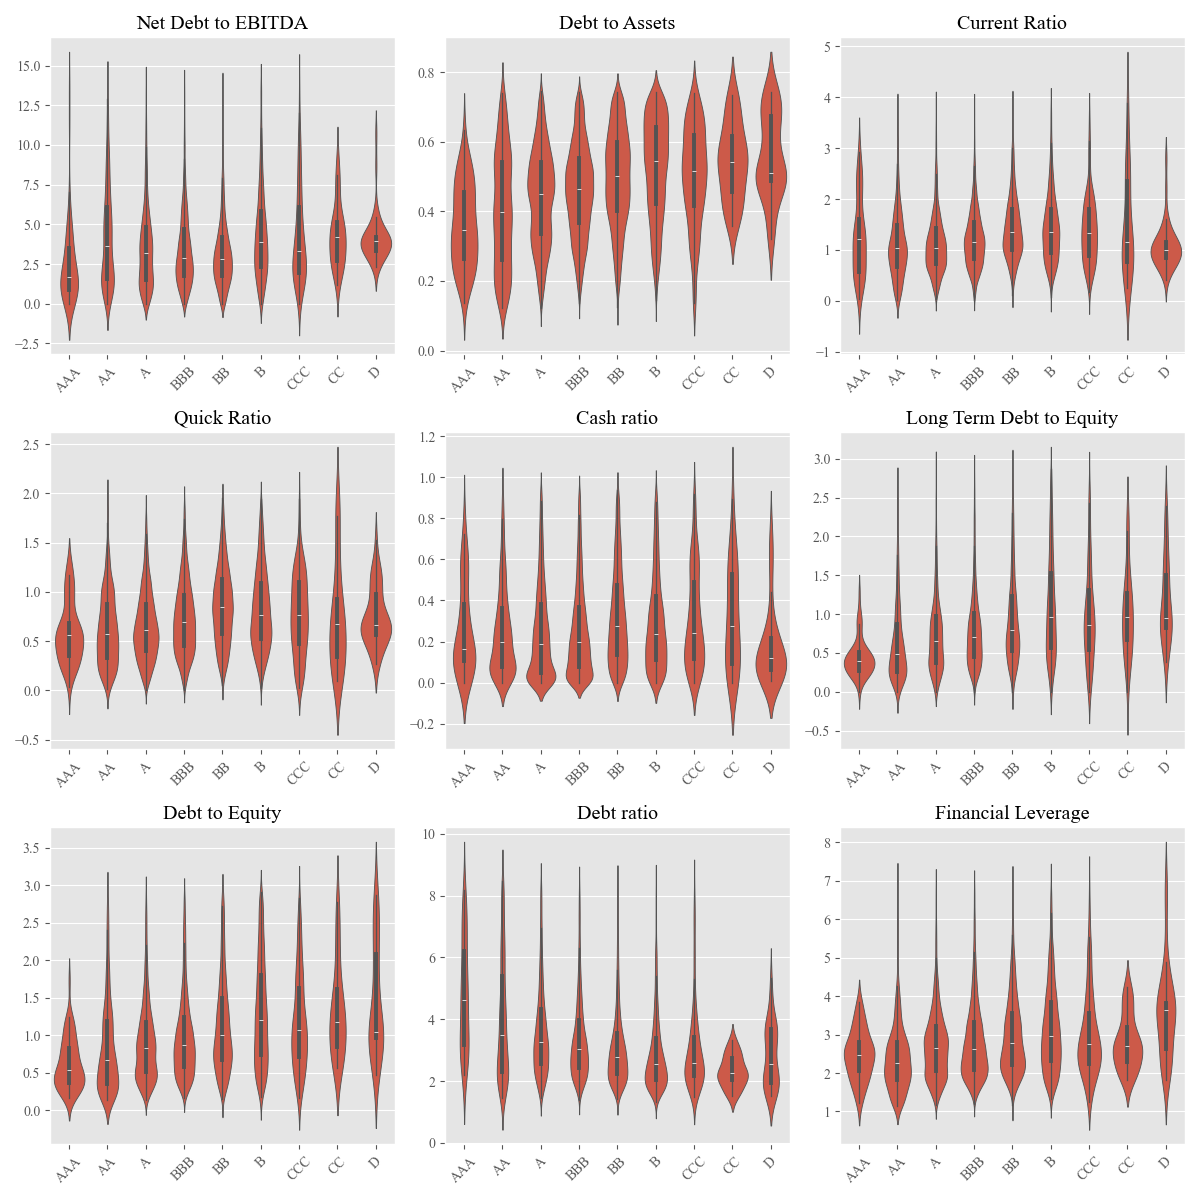
\includegraphics[width=0.91\textwidth]{distribution_metricas_por_rating.png}
\caption{Distribución de las métricas por Rating}
\label{fig:dist_met_rat}
\end{figure}

Mencionar que para un primer análisis hemos agrupado los Rating por una categoría más amplia que la oficial, Cuadro \ref{tab:credit-ratings}. Empleando la misma aproximación, también hemos podido observar que esta misma diferencia de distribuciones en las métricas se puede observar para cada Sector, indicándonos que es una variable relevante a tener en cuenta. 

Para poder emplear los diferentes modelos de regresión y clasificación, nuestras dos variables categóricas las hemos transformado en variables numéricas asignado un numero a cada sector y para el caso del Rating asignado un 0 a la categoría AAA, un 1 a la AA+ y así sucesivamente.

Es importante destacar cómo se distribuyen las compañías por rating, ya que como se observa en la Figura \ref{fig:dist_rat_sec}, los Ratings siguen una distribución que tiende a concentrarse alrededor del Rating BBB. Este hecho nos obliga a realizar un muestreo ponderado (\textit{oversampling}) de los datos para garantizar que nuestro modelo no esté sesgado hacia las categorías más frecuentes.

\begin{figure}
\centering
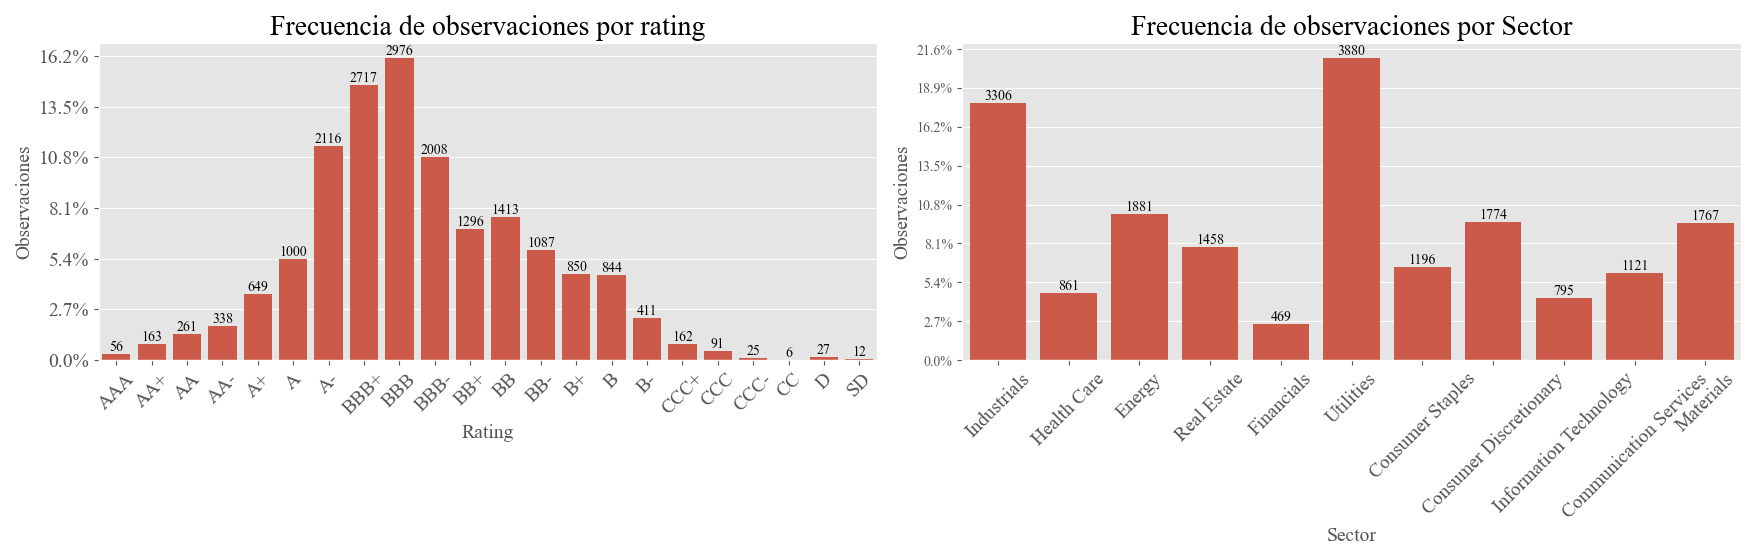
\includegraphics[width=0.92\textwidth]{distribution_rating_sectores.png}
\caption{Distribución de los Ratings y los sectores}
\label{fig:dist_rat_sec}
\end{figure}

El \textit{oversampling} los hemos realizado tanto sobre la clasificación de Ratings proporcionada por las agencias como sobre nuestra categorización más general, permitiendo así que los modelos manejen de manera más equitativa las diversas categorías de Rating.

La siguiente sección, \ref{sec:analsis_previos}, detallará los cálculos y el análisis estadístico previos a la implementación de los modelos, que se explorarán y analizarán en la Seccion \ref{sec:resultados}, con el objetivo de identificar el modelo que mejor se ajuste a los datos y proporcione las estimaciones más precisas del rating.

\newpage
\subsection{Análisis previos}\label{sec:analsis_previos}

Antes de desarrollar nuestros modelos de regresión, es fundamental validar ciertas hipótesis sobre nuestros datos, ya que los modelos de regresión asumen condiciones específicas que deben ser verificadas para asegurar la validez de las conclusiones del modelo. Los datos empleados deben cumplir los siguientes supuestos:

\begin{enumerate}
    \item Sólo la variable dependiente \(Y\) se trata como aleatoria.
    \item Las observaciones de \(Y=(y_1, y_2, \ldots, y_n)\) deben ser independientes. Esta hipótesis generalmente se cumple, ya que las compañías en nuestra muestra son en su gran mayoría independientes entre sí.
    \item Para cada individuo en la muestra se cumple que \(y_i = b_0 + b_1 x_i + u_i\), donde \(u_i\) es una perturbación aleatoria o residuo.
    \item Homoscedasticidad: la varianza de \(Y\) es constante respecto de \(X\). Observaremos más adelante que esta condición no se cumple en nuestros datos.
    \item Normalidad de la variable \(Y\). Aunque hemos observado en la Figura \ref{fig:freq_rat} que \(Y\) sigue aproximadamente una distribución normal, realizaremos pruebas adicionales para confirmarlo.
\end{enumerate}

\subsubsection{Contrastes de Hipótesis}
Las pruebas de hipótesis se utilizan para determinar si existen diferencias estadísticamente significativas entre grupos o condiciones. Dependiendo de la independencia, normalidad de los datos y tamaño de muestra, consideramos las siguientes opciones:

\begin{enumerate}
    \item Si los datos son independientes y siguen una distribución normal o el tamaño de muestra es mayor o igual a 30, utilizamos la prueba T de Student para datos independientes. Primero, comparamos las varianzas con una prueba adecuada.
    \item Si los datos son independientes, no siguen una distribución normal y el tamaño de la muestra es menor que 30, utilizamos pruebas no paramétricas.
    \item Para datos apareados que siguen una distribución normal o si el tamaño de muestra es mayor o igual a 30, aplicamos la prueba T de Student para datos apareados.
    \item Para datos apareados que no siguen una distribución normal y el tamaño de muestra es menor que 30, se recomiendan pruebas no paramétricas, como la prueba T de Wilcoxon.
\end{enumerate}

\subsubsection{Verificación de la Normalidad}
Verificar la normalidad de la distribución es esencial para muchas pruebas estadísticas. Utilizamos varias técnicas para evaluar la normalidad:

\begin{enumerate}
    \item Representar los datos en papel probabilístico. Se trata de un gráfico de dispersión que compara los valores observados con los que esperaríamos encontrar si la distribución fuera Normal. Si los puntos siguen una recta diagonal los datos siguen una distribución Normal. Como se puede observar en la Figura \ref{fig:qqplot}, los datos no muestras un distribución normal, salvo en el caso de la variable dependiente. 
    
    \begin{figure}
    \centering
    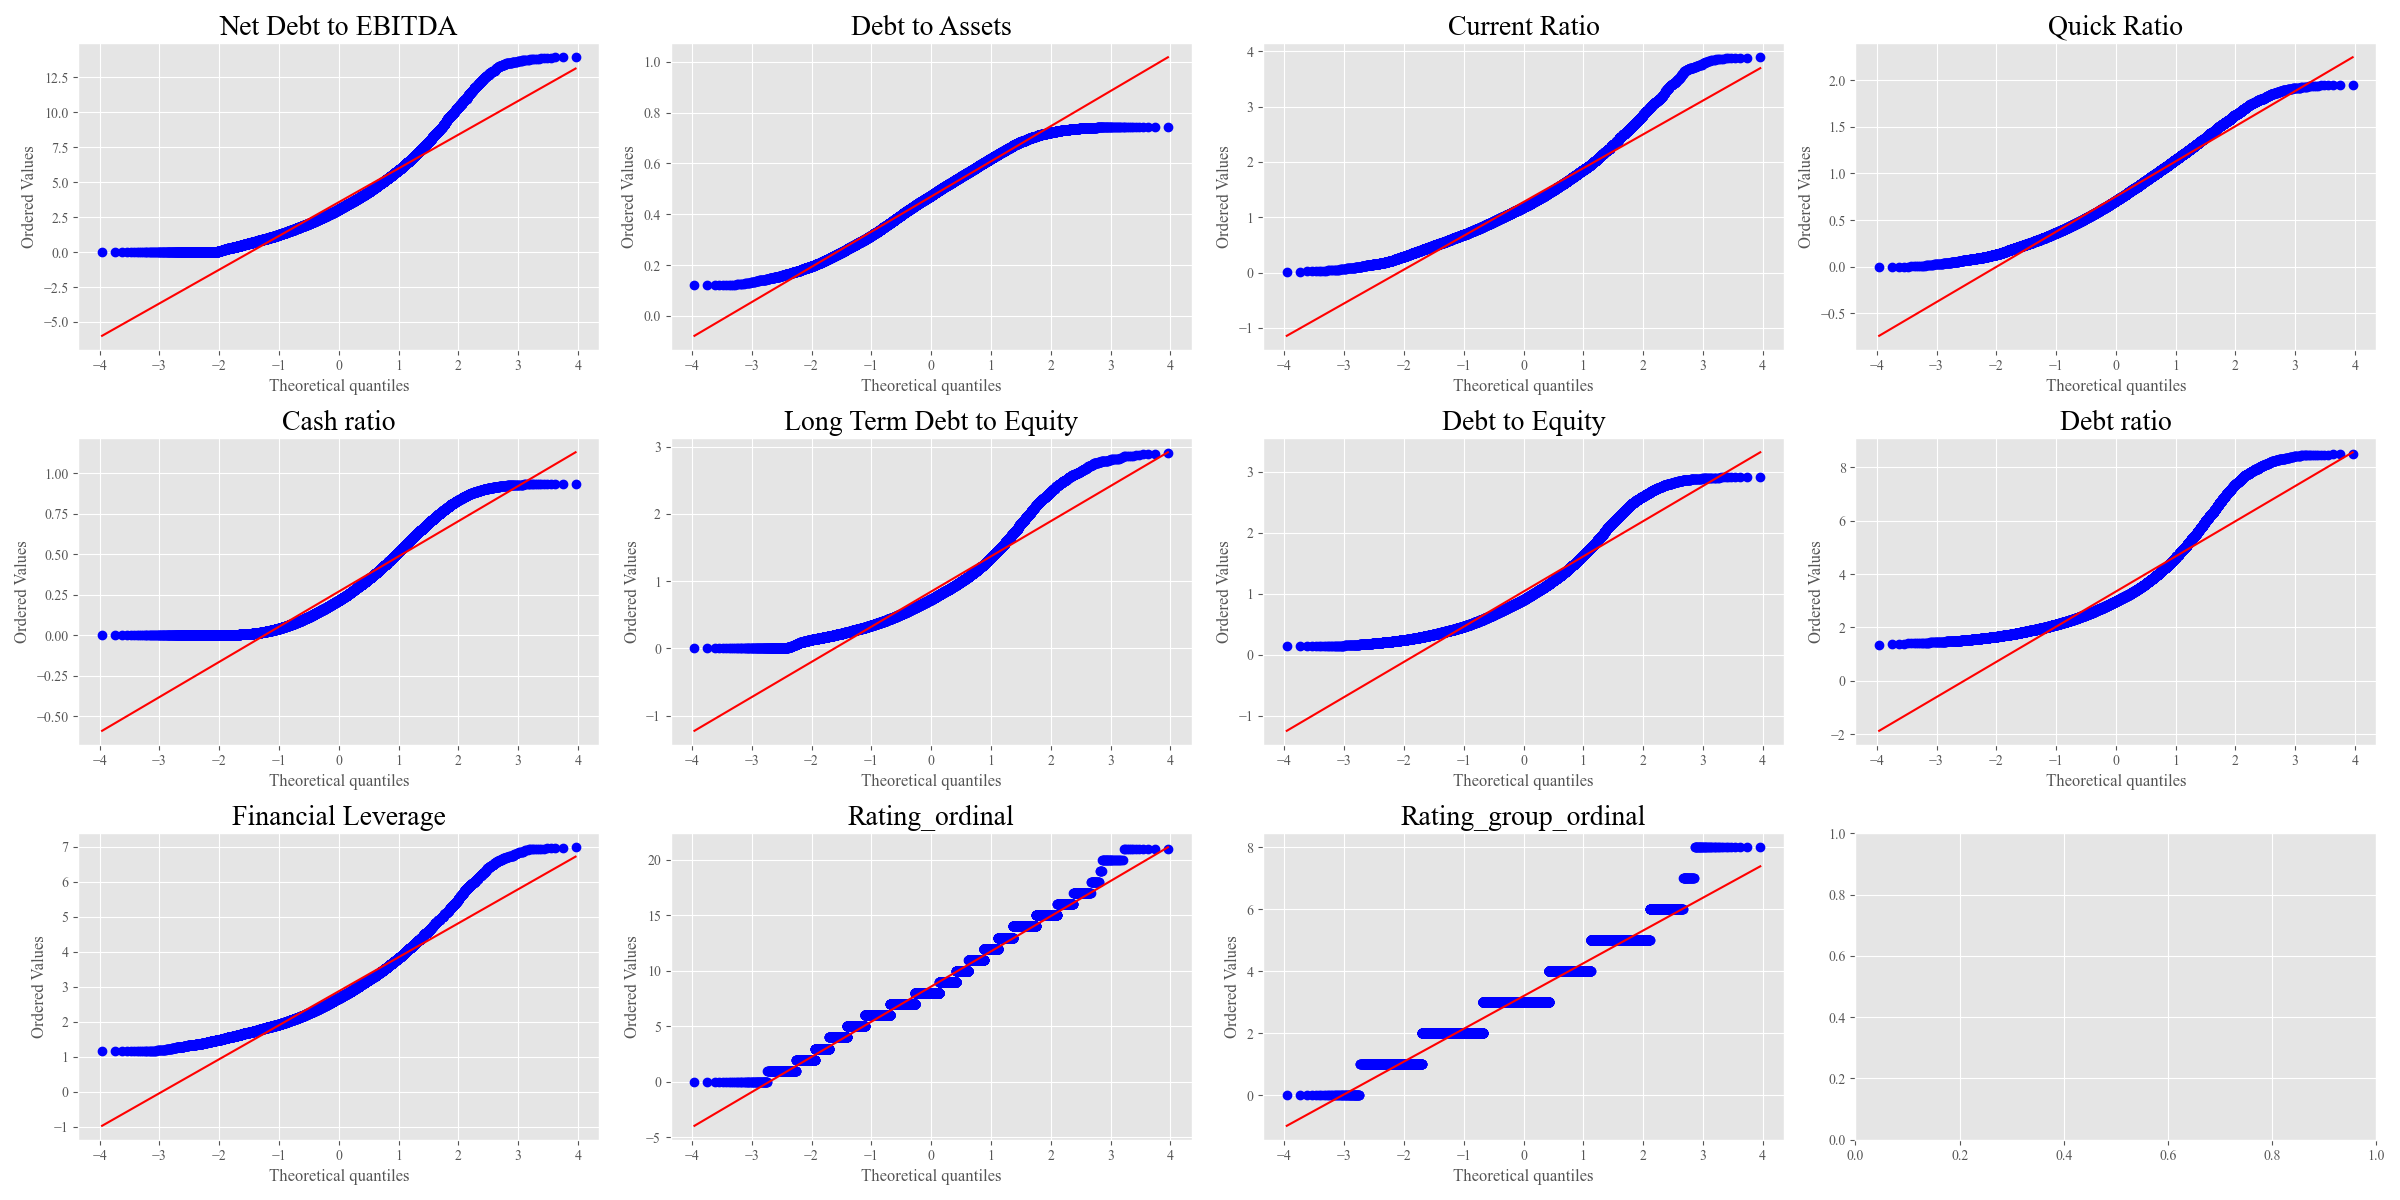
\includegraphics[width=0.95\textwidth]{qqplot.png}
    \caption{QQ plot de todas la variables}
    \label{fig:qqplot}
    \end{figure}
    
    \item Representar un histograma y comprobar la forma de campana. Esto se puede observar en la Figura \ref{fig:histogram}, donde además de la variable independiente observamos que la métrica Debt to Asset también sigue una variable prácticamente normal.

    \begin{figure}
    \centering
    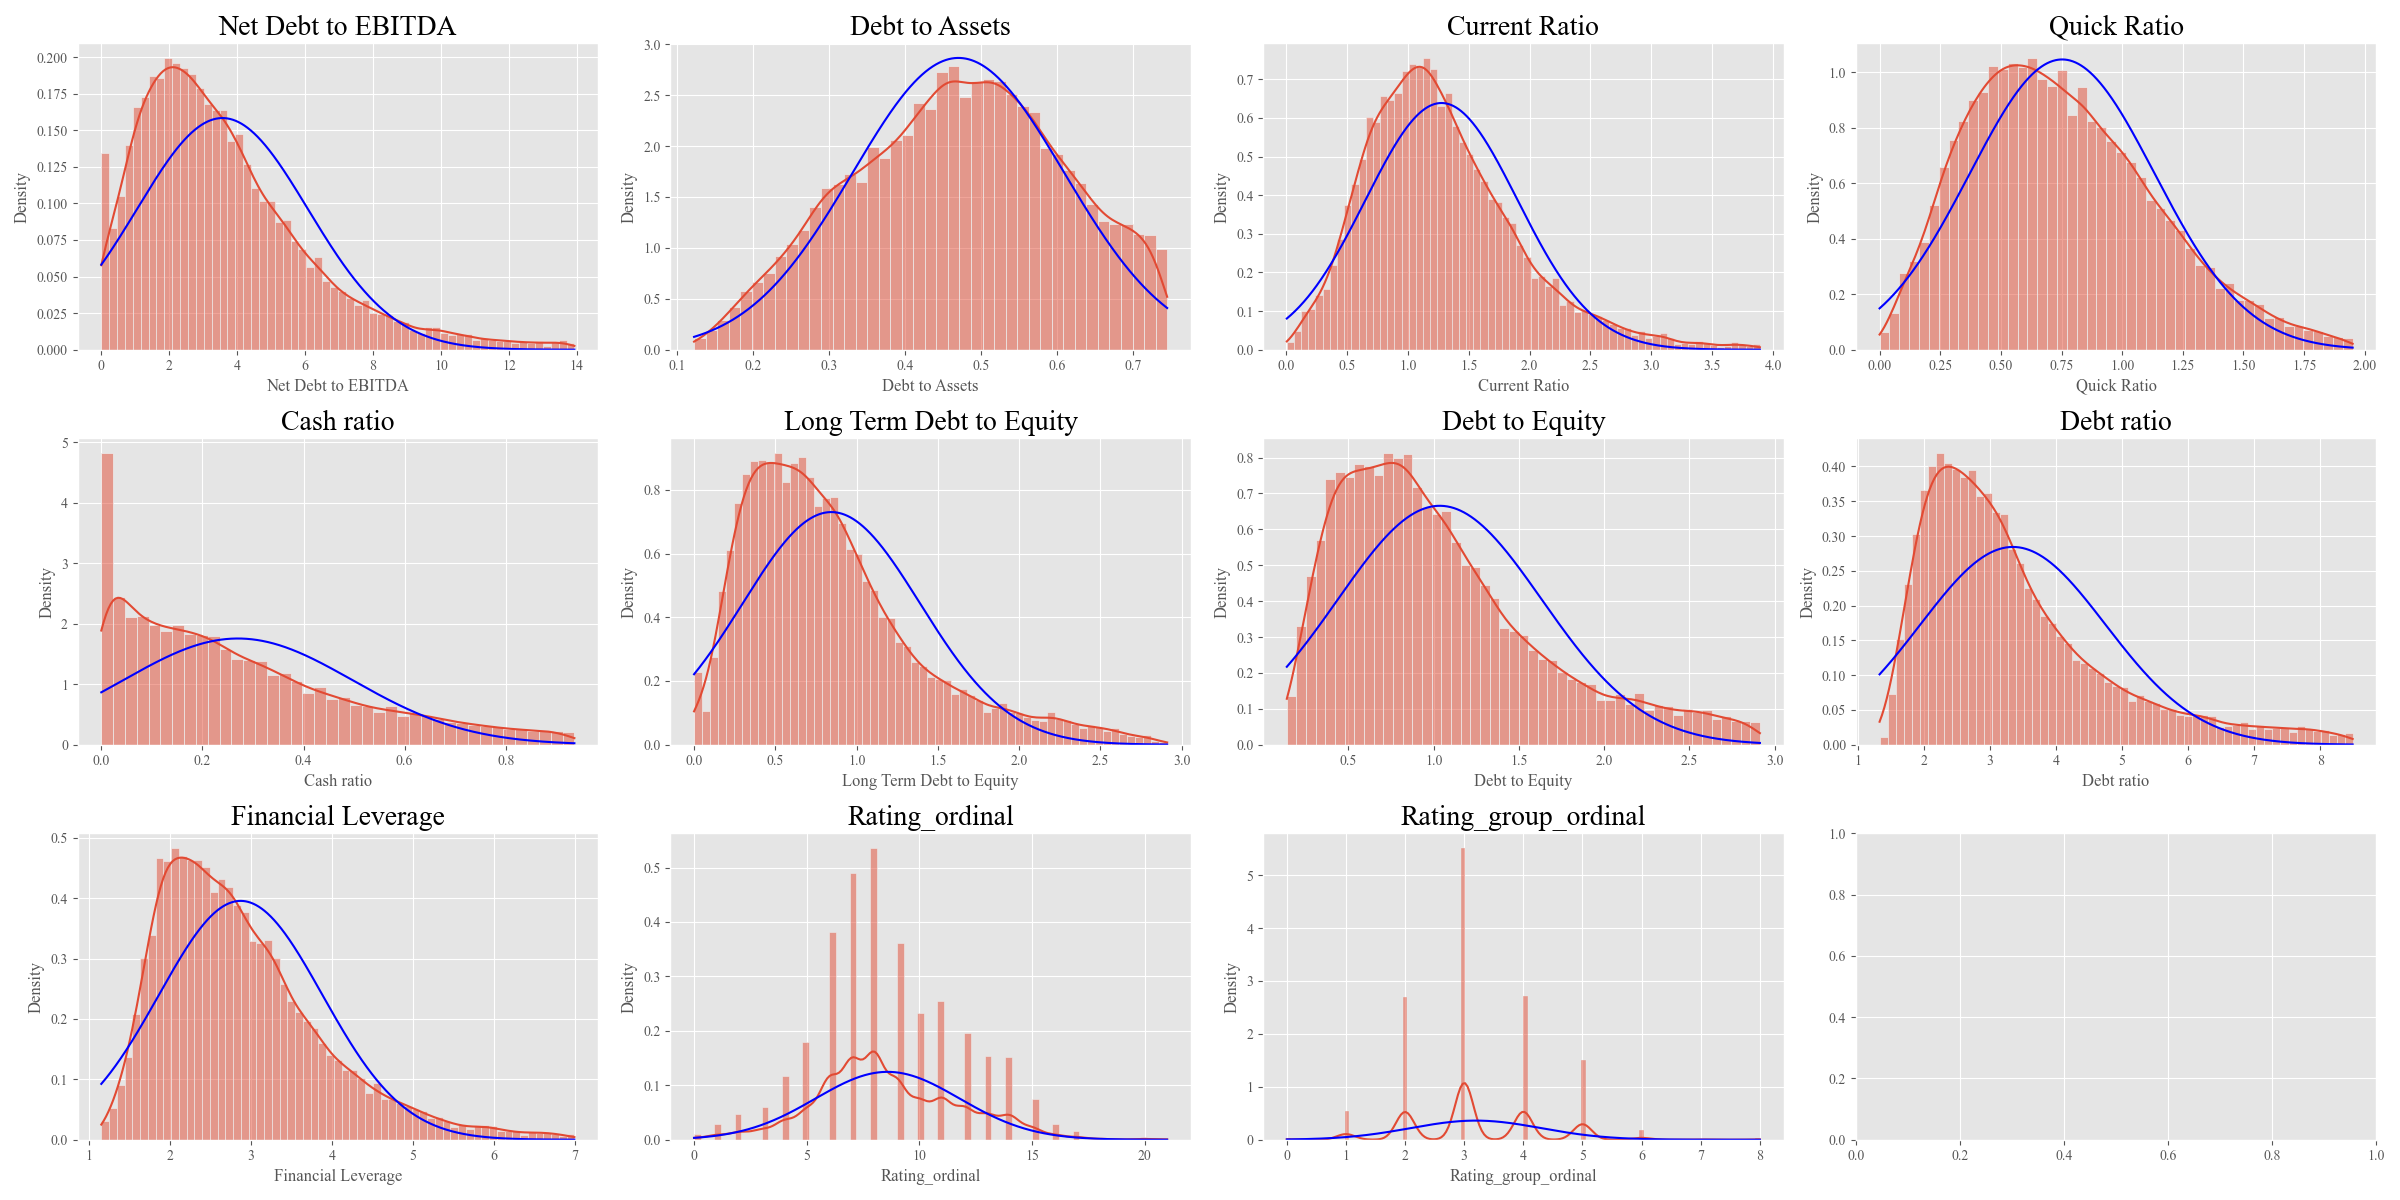
\includegraphics[width=0.95\textwidth]{histogram.png}
    \caption{Histograma de todas las variables}
    \label{fig:histogram}
    \end{figure}
    
    \item Comprobar que la distribución es simétrica y mesocúrtica. Se puede hacer comprobando que los coeficientes de asimetría (CA) y de apuntamiento o curtosis (CC) no son significativamente diferentes de 0 mediante sus intervalos de confianza del 95\%, o bien comprobando que los coeficientes tipificados de asimetría y curtosis están comprendidos entre ±2. Este análisis se puede comprobar en la Tabla \ref{tab:dist_sim_mes}

    \begin{table}
        \centering
        \begin{tabular}{|l|P{2.3cm}|P{2cm}|P{2.5cm}|P{3cm}|}
        \hline
        \textbf{Métrica}  & \textbf{Coeficiente de asimetría} & \textbf{Coeficiente de curtosis} & \textbf{Simetría} & \textbf{Mesocúrtica} \\ \hline
        Net Debt to EBITDA & 1.20 &  1.67 & No es simétrica & No es mesocúrtica \\
        Debt to Assets & -0.12 & -0.70 & No es simétrica & No es mesocúrtica \\
        Current Ratio & 0.92 &  1.17 & No es simétrica & No es mesocúrtica \\
        Quick Ratio & 0.53 & -0.16 & No es simétrica & No es mesocúrtica \\
        Cash ratio                & 0.90 &  0.05 & No es simétrica & No es mesocúrtica \\
        Long Term Debt to Equity  & 1.14 &  1.17 & No es simétrica & No es mesocúrtica \\
        Debt to Equity            & 0.99 &  0.50 & No es simétrica & No es mesocúrtica \\
        Debt ratio                & 1.34 &  1.59 & No es simétrica & No es mesocúrtica \\
        Financial Leverage        & 1.09 &  1.29 & No es simétrica & No es mesocúrtica \\
        Rating & 0.32 &  0.16 & No es simétrica & No es mesocúrtica \\
        Rating agrupado & 0.38 &  0.56 & No es simétrica & No es mesocúrtica \\ \hline
        \end{tabular}
        \caption{Comprobación de distribución simétrica y mesocúrtica}
        \label{tab:dist_sim_mes}
    \end{table}
    
    \item Utilizar pruebas de bondad de ajuste como la prueba de Kolmogorov-Smirnov (K-S). Se basan en comparar la distribución acumulada de los valores de la muestra observada con la distribución acumulada que se obtendría en el supuesto que siguiera una distribución Normal con la misma media y varianza. Si en la prueba de K-S se obtienen valores de $p<5\%$, la distribución difiere significativamente de una Normal. Dado que tenemos una serie de datos mayor a 5000, el librería de Python \textit{scipy} recomienda usar el Test de Lilliefors, el cual es un tipo de test de Kolmogorov-Smirnov. Realizando este test para nuestras variables independientes tampoco obtenemos una distribución normal de los datos, con un nivel de significativdad del $1\%$.
\end{enumerate}

\subsubsection{Homocedasticidad}
Nuestro siguiente paso es comprobar la homocedasticidad de los datos. Dado que los datos ya hemos comprobado que no se comportan de manera normal usaremos el test de Levene. El test de Levene pone a prueba la hipótesis nula de que todas las muestras proceden de poblaciones con varianzas iguales y es una alternativa en el caso de que haya desviaciones significativas de la normalidad. 

Cuando obtienes p-valores menores a 0.05 en la prueba de Levene, indica que las varianzas entre tus grupos no son iguales, es decir, tus datos violan la suposición de homocedasticidad. Esto afecta el uso de pruebas paramétricas que asumen igualdad de varianzas entre los grupos, como el t-test para muestras independientes y la ANOVA.  Aplicar transformaciones a tus datos puede ayudar a estabilizar la varianza. Algunas transformaciones que hemos intentado para poder ajustar los datos son:

\begin{enumerate}
    \item Logarítmica: $\log{x}$ es útil para datos con varianzas que aumentan con la media.
    \item Raíz Cuadrada: $\sqrt{x}$ para datos de conteo o tasas.
    \item Box-Cox: La transformación Box-Cox puede ser aplicada a datos positivos y busca una transformación que estabilice la varianza y aproxime los datos a una distribución normal.
\end{enumerate}

\noindent Después de probar estas tres técnicas no hemos conseguido mejorar la la homocedasticidad y por tanto asumiremos que nuestros datos tiene heterocedasticidad (las varianzas son diferentes entre los grupos).

\subsubsection{Comparación de medias entre muestras}
Una vez vemos que no son normales y no tienen varianzas homogéneas, debemos considerar el uso de métodos no paramétricos para nuestros análisis, como la prueba de Kruskal-Wallis para comparar medianas en lugar de medias. Realizando este análisis para las 9 métricas, obtenemos que hay diferencias estadísticamente significativas entre las medias de los Ratings, con un nivel de significatividad del 5\%.

Una vez que has determinado que existen diferencias significativas entre los grupos mediante la prueba de Kruskal-Wallis, el siguiente paso es realizar un análisis post-hoc para identificar específicamente entre qué pares de grupos existen esas diferencias. La Prueba de Dunn es una opción popular para comparaciones múltiples después de una Prueba de Kruskal-Wallis, ya que está diseñada para datos no paramétricos. La Figura \ref{fig:dunn_pvalues}, nos dice que para los cuadrantes donde el p-value es proximoa 0 (es decir blanco) las medias de las muestras son diferentes. Es decir, las medias de los datos con Rating peores (entorno al CC) son significativamente diferentes del resto

\begin{figure}
\centering
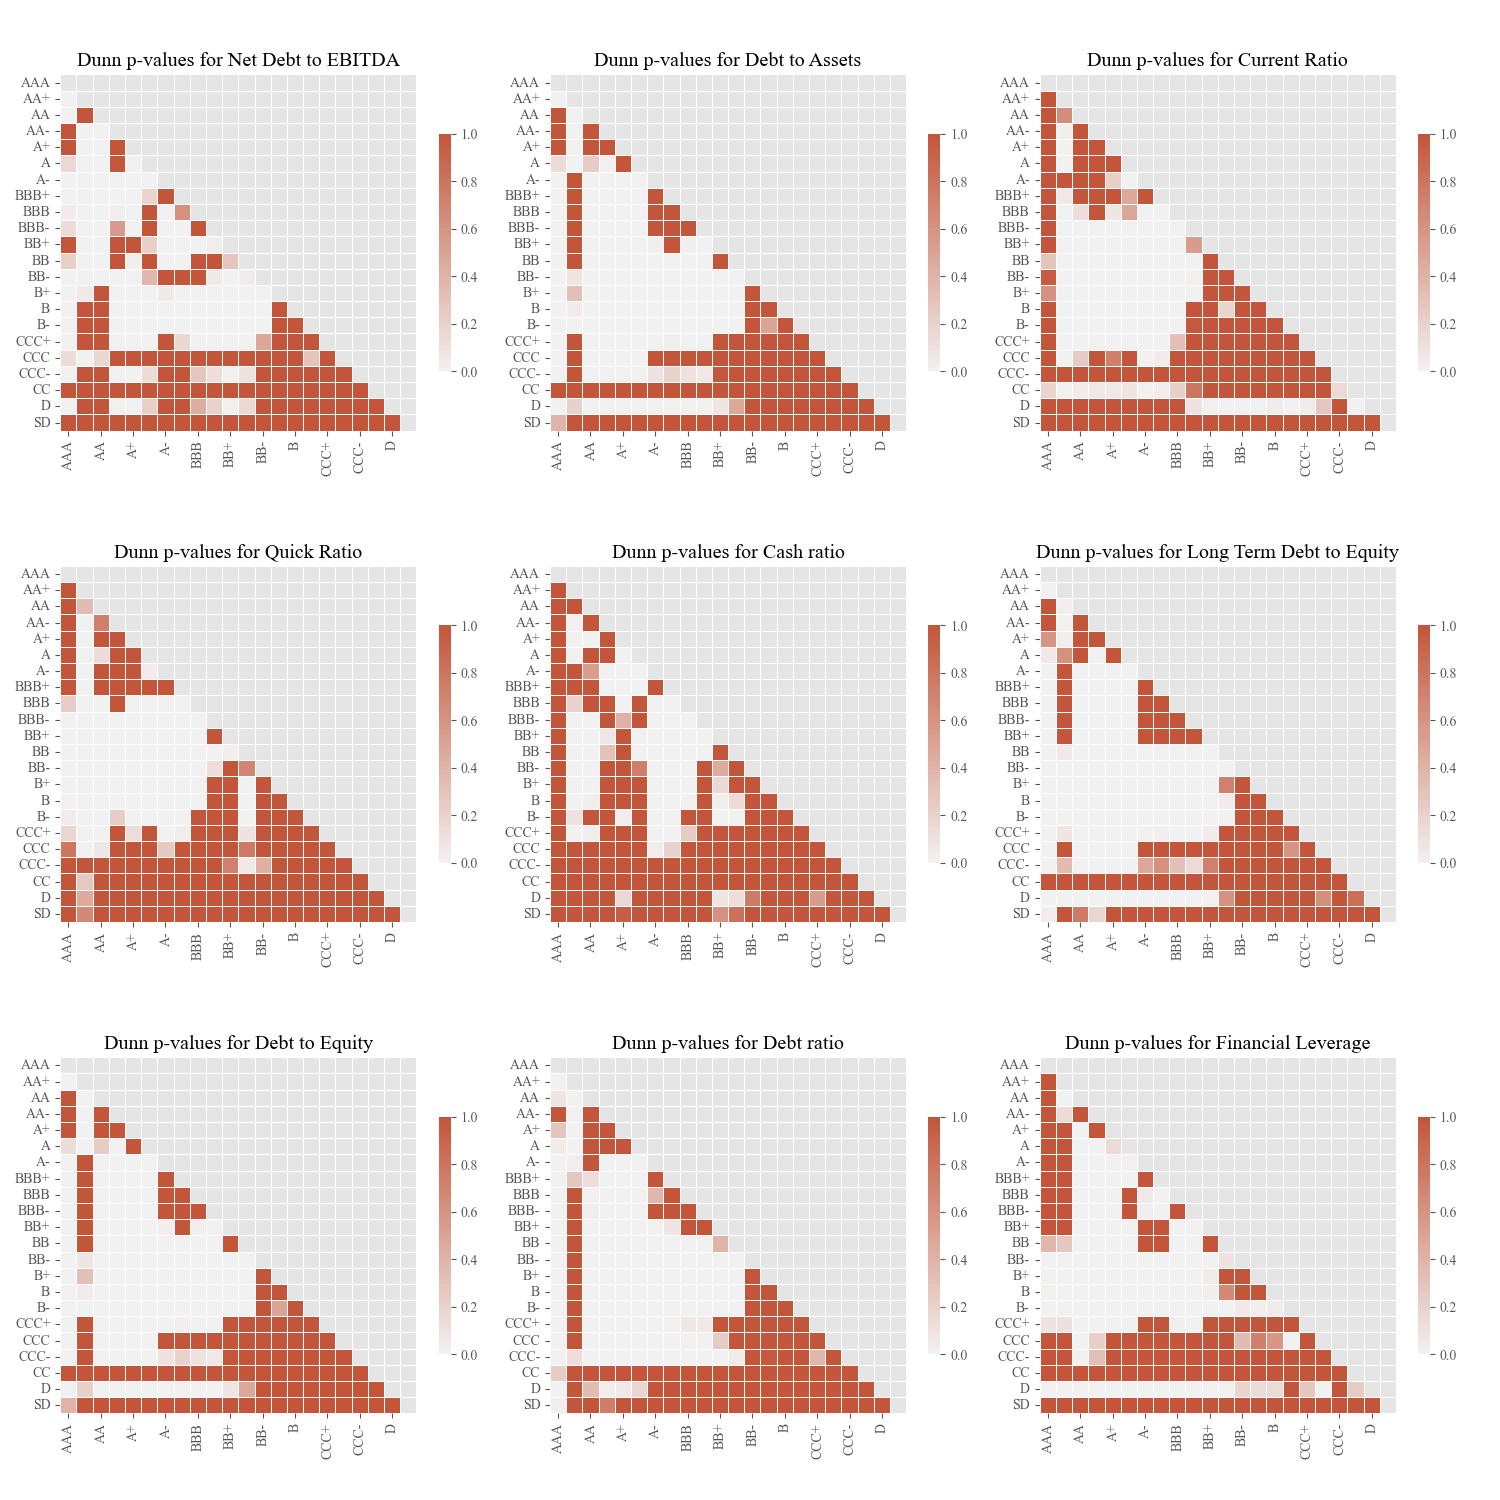
\includegraphics[width=1\textwidth]{dunn_pvalues.png}
\caption{P-Values obtenidos de la prueba de Dunn}
\label{fig:dunn_pvalues}
\end{figure}

\subsubsection{Colinealidad}
Examinamos la colinealidad entre las variables utilizando una muestra aleatoria de datos. La Figura \ref{fig:pairplot} muestra estas relaciones, indicando posibles redundancias entre variables que podrían afectar la eficacia de los modelos de regresión. 

\begin{figure}
\centering
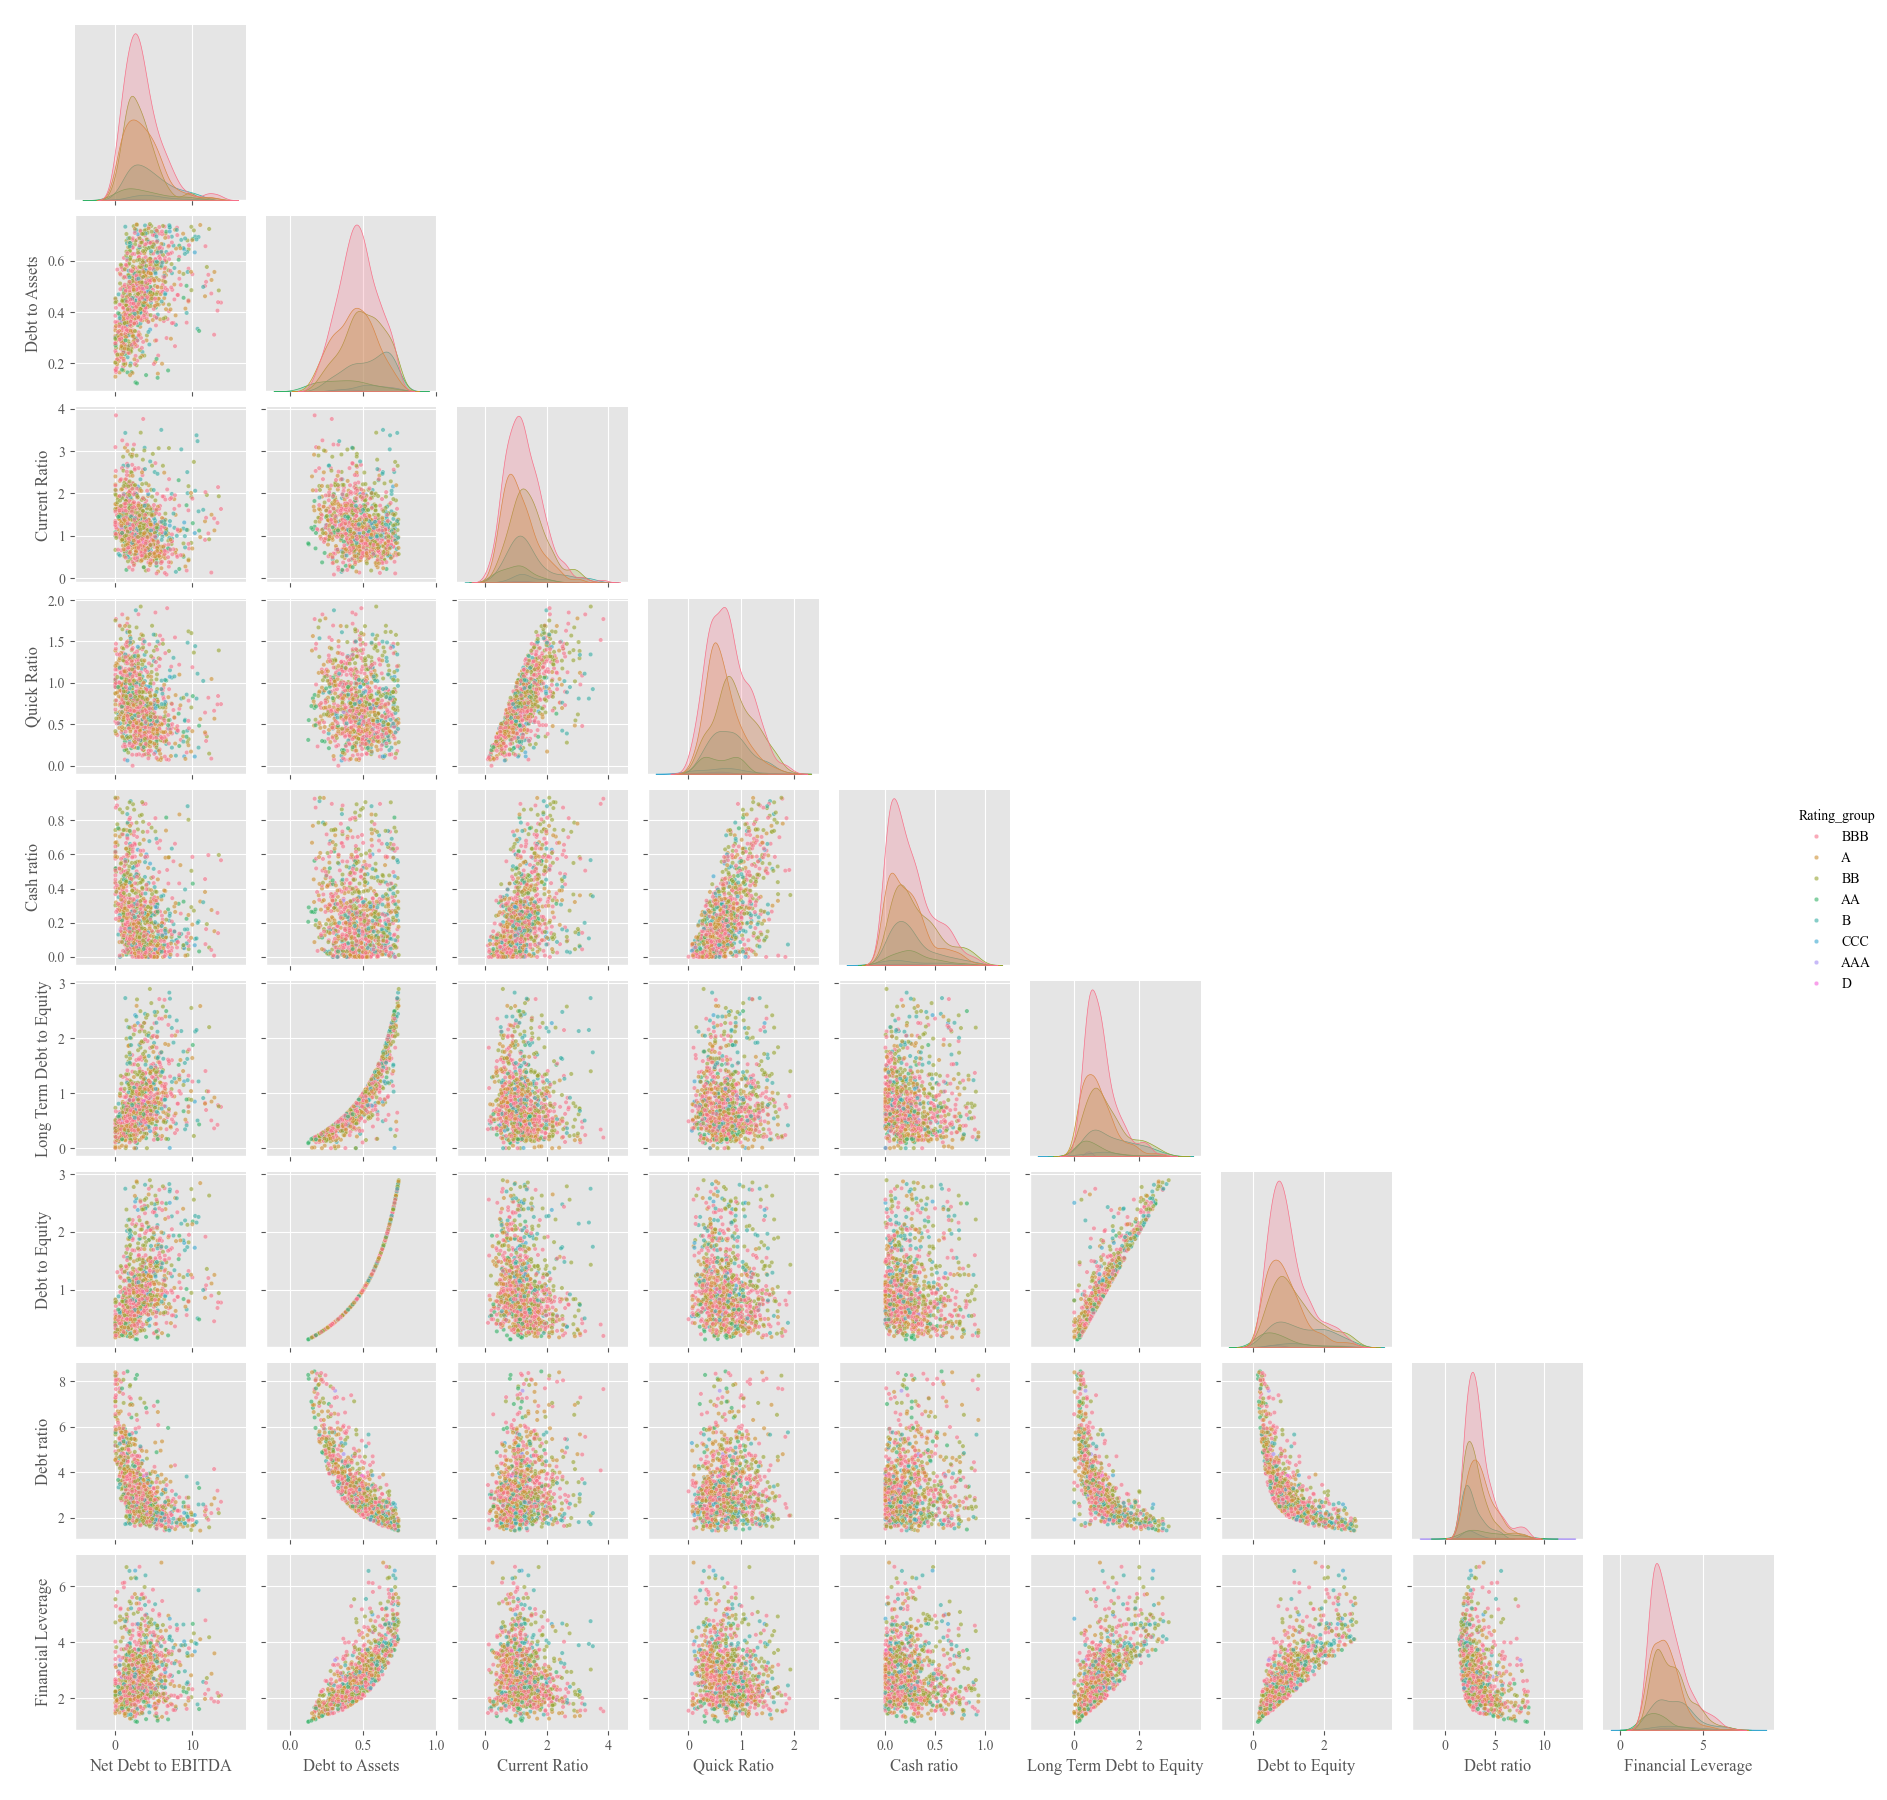
\includegraphics[width=1\textwidth]{pairplot.png}
\caption{Diagrama de dispersión para examinar la colinealidad entre variables}
\label{fig:pairplot}
\end{figure}

\subsubsection{Correlación entre variables}
Para asegurarnos que la correlación es significativa realizaremos diferentes contrastes de hipótesis. En nuestro caso, donde ya hemos visto que  las variables no siguen una distribución normal, utilizamos medidas de correlación no paramétricas como Spearman o Kendall. Estas medidas son adecuadas para datos ordinales o distribuciones no normales y son esenciales para evaluar la relación entre variables antes de la modelización. En la Figure \ref{fig:heatmap_correlation} observamos la matriz de correlaciones de Spearman.

\begin{figure}
\centering
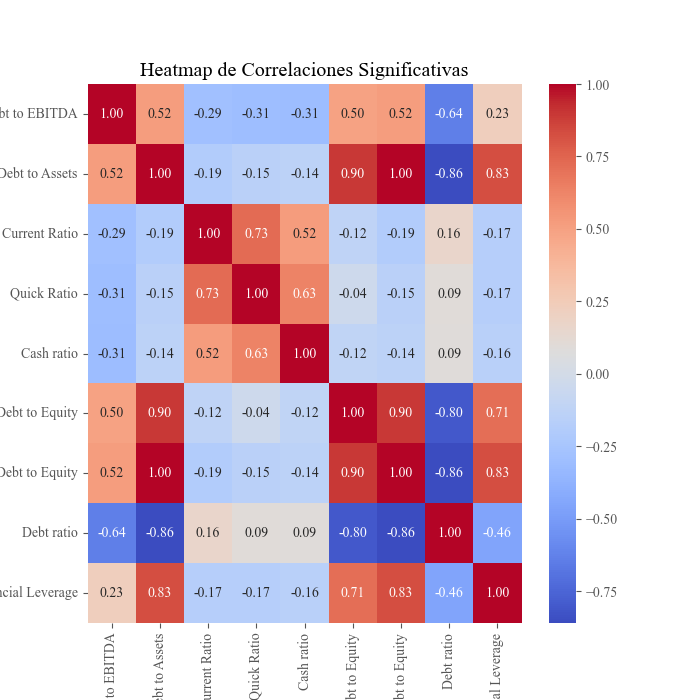
\includegraphics[width=0.5\textwidth]{heatmap_correlation.png}
\caption{Matriz de significativadad de correlaciones}
\label{fig:heatmap_correlation}
\end{figure}

Sin embargo aunque obtengamos que todas las variables están correlacionadas significativamente esto no quiere decir que tengamos que quedarnos solo con una variable a la hora de hacer el modelo. Como veremos en el caso más sencillo de clasificación la combinación de estas variables funciona mucho mejor que una única variable. Esto puede deberse a varios motivos:

\begin{itemize}
\item Efectos combinados y sinergias: Cuando usas todas las variables juntas en una regresión, el modelo puede capturar efectos combinados y sinergias entre las variables que no son evidentes cuando las variables se modelan de manera individual. Esto significa que algunas variables pueden tener un efecto significativo en la variable dependiente solo cuando se consideran en conjunto con otras variables.
\item Control de variables confusas: En un modelo de regresión múltiple, incluir múltiples predictores puede ayudar a controlar el efecto de variables confusas. Esto puede hacer que las estimaciones de los coeficientes para las variables de interés sean más precisas y menos sesgadas que en análisis univariados.
\item Multicolinealidad: Aunque la multicolinealidad generalmente se considera un problema, en algunos casos puede hacer que el modelo completo funcione mejor en términos de predicción. Esto se debe a que las variables altamente correlacionadas pueden reforzarse entre sí para mejorar la capacidad predictiva del modelo.
\item Capacidad predictiva vs. significancia estadística: La significancia estadística de las correlaciones individuales no siempre se traduce directamente en una alta capacidad predictiva. Un modelo puede ser estadísticamente significativo y tener buenos p-valores para las pruebas de hipótesis, pero esto no garantiza que tendrá un buen rendimiento predictivo cuando se aplique a nuevos datos. Por otro lado, un modelo de regresión múltiple puede no tener todas sus variables significativas individualmente, pero como conjunto, puede predecir muy bien la variable de interés
\end{itemize}

En resumen, este análisis preliminar es crucial para asegurar que los datos estén preparados adecuadamente para los modelos de regresión y que las suposiciones subyacentes de las técnicas estadísticas se cumplan.


\section{Modelos}\label{sec:modelos}

En este aparado probaremos los modelos de regresión y clasificación que hemos considerado más adecuados. Desde los modelos más básicos de clasificación hasta algoritmos de ML como el Random Forest.

Antes de realizar los test estadísticos de las variables dependientes analizaremos las frecuencias de los datos para cada Rating. Como observamos en la Figura \ref{fig:freq_rat}, observamos para la mayoría de las métricas tienen diferencias en las frecuencias de los datos para cada Rating. Esto nos ayudará a obtener mejores predicciones con nuestros modelos.

\begin{figure}[H]
\centering
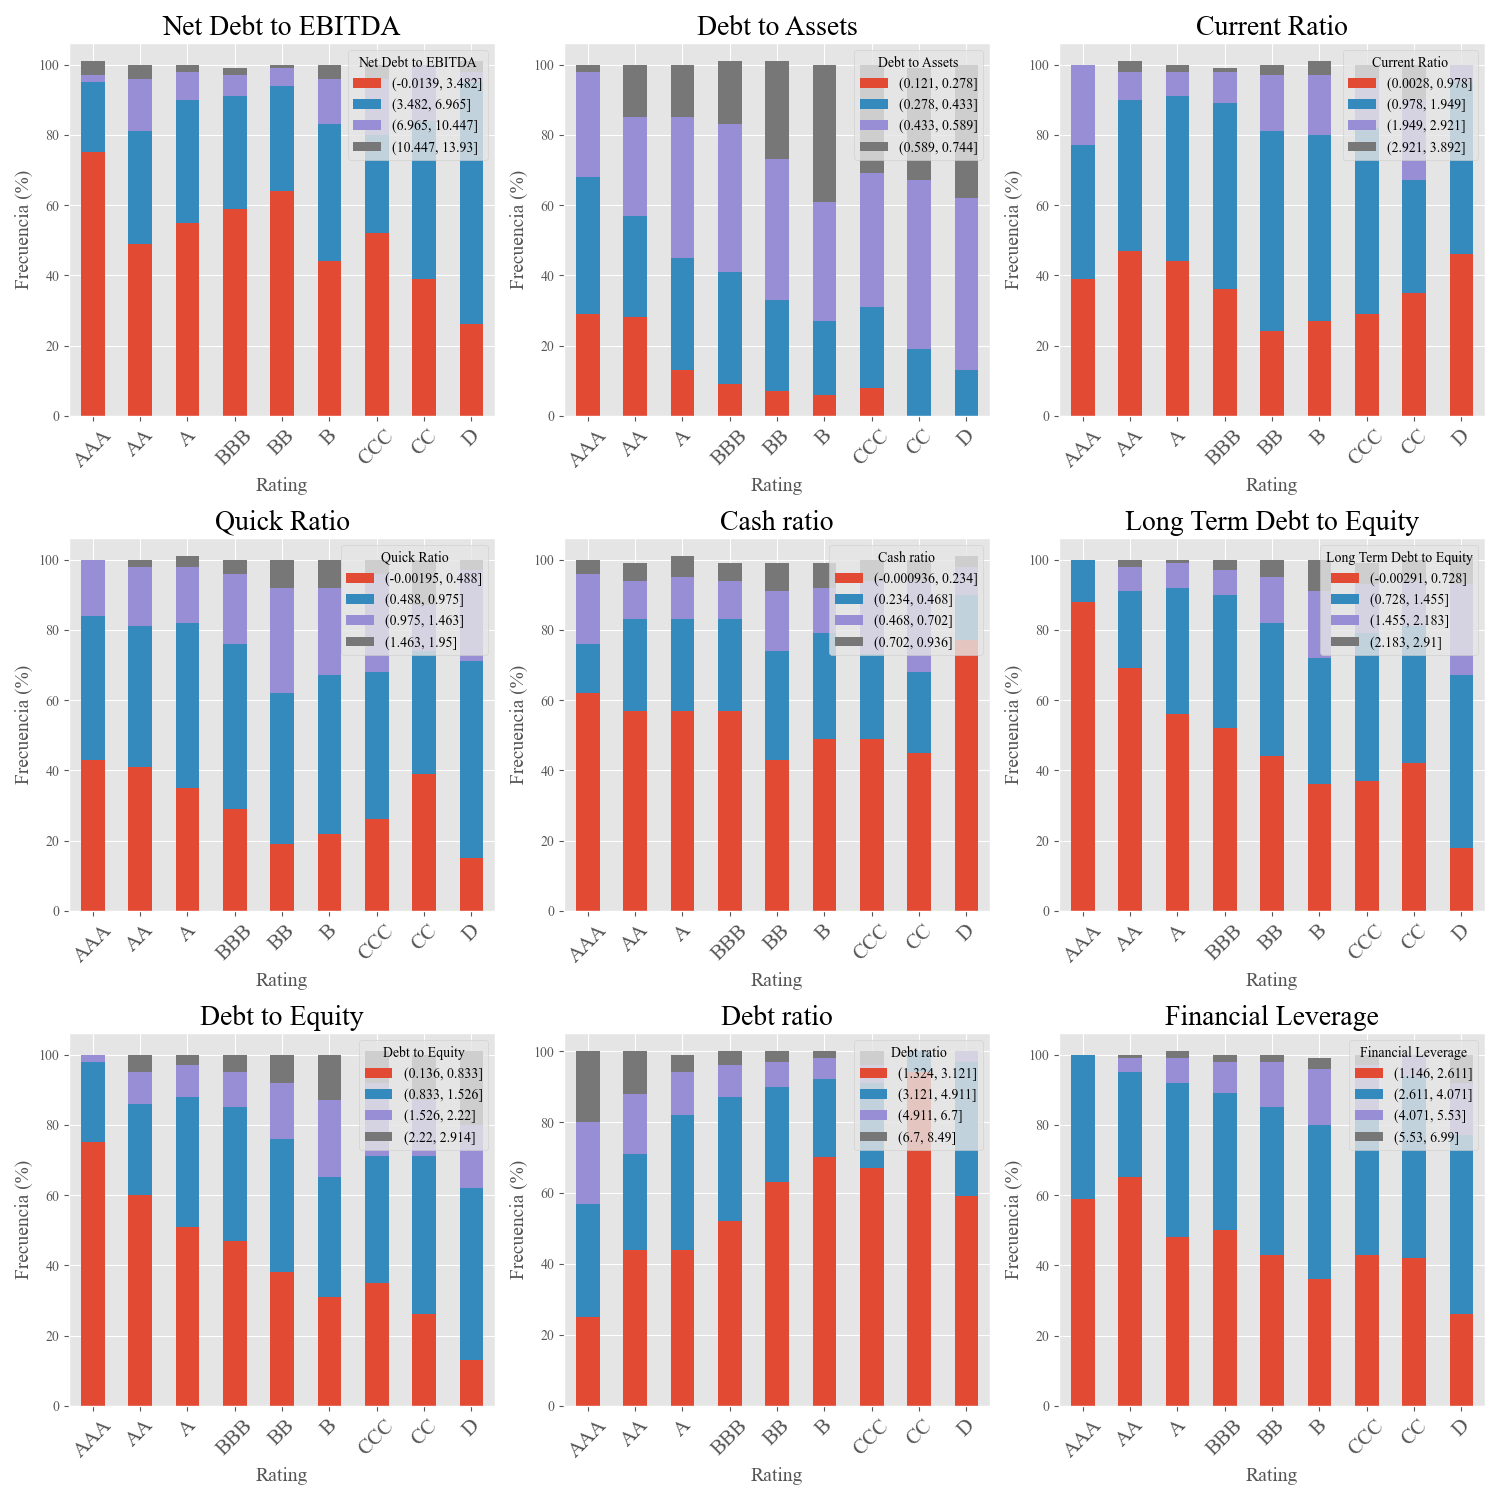
\includegraphics[width=0.95\textwidth]{frecuencias_por_rating.png}
\caption{Frecuencia de las métricas por Rating}
\label{fig:freq_rat}
\end{figure}

\subsection{Modelos de clasificación Lineal}
El modelo más sencillo de clasificación consiste en, dada la métrica $i$, el Rating estimado sería el Rating el cual tenga su medía más cercana, es decir, para un valor \( x \) y un conjunto de medias \( M = \{m_1, m_2, \ldots, m_n\} \), calculamos la diferencia absoluta entre \( x \) y cada \( m_i \) en \( M \), generando un conjunto \( D \) de diferencias:

\[
D = \{|x - m_1|, |x - m_2|, \ldots, |x - m_n|\}
\]

% Encontrar el índice de la diferencia mínima
Buscamos el índice \( k \) tal que \( D_k \) es el mínimo en \( D \), donde \( D_k = |x - m_k| \) es la diferencia mínima absoluta entre \( x \) y las medias en \( M \). Matemáticamente, esto los podemos expresar como:

\[
k = \underset{i}{\mathrm{argmin}} \, |x - m_i|
\]

Donde \( \mathrm{argmin} \) devuelve el índice \( i \) del elemento de \( M \) que minimiza la diferencia absoluta con \( x \), esencialmente encontrando la media más cercana a \( x \) según la diferencia absoluta. 

Este análisis lo realizamos para una de las 9 métricas y luego de manera conjunta, es decir, haciendo la media de los resultados de las 9 clasificaciones. Para observar los resultados obtenidos, hemos hecho una matriz de confusión para cada caso. Como se puede observar en la Figura \ref{fig:confusion_matrix_por_metrica}, los resultados cuando lo vemos métrica a métrica no son buenos, pero con la media de los 9 resultados, el Error Cuadratico Medio o Mean Square Error (MSE) mejoró considerablemente.

\begin{figure}[H]
\centering
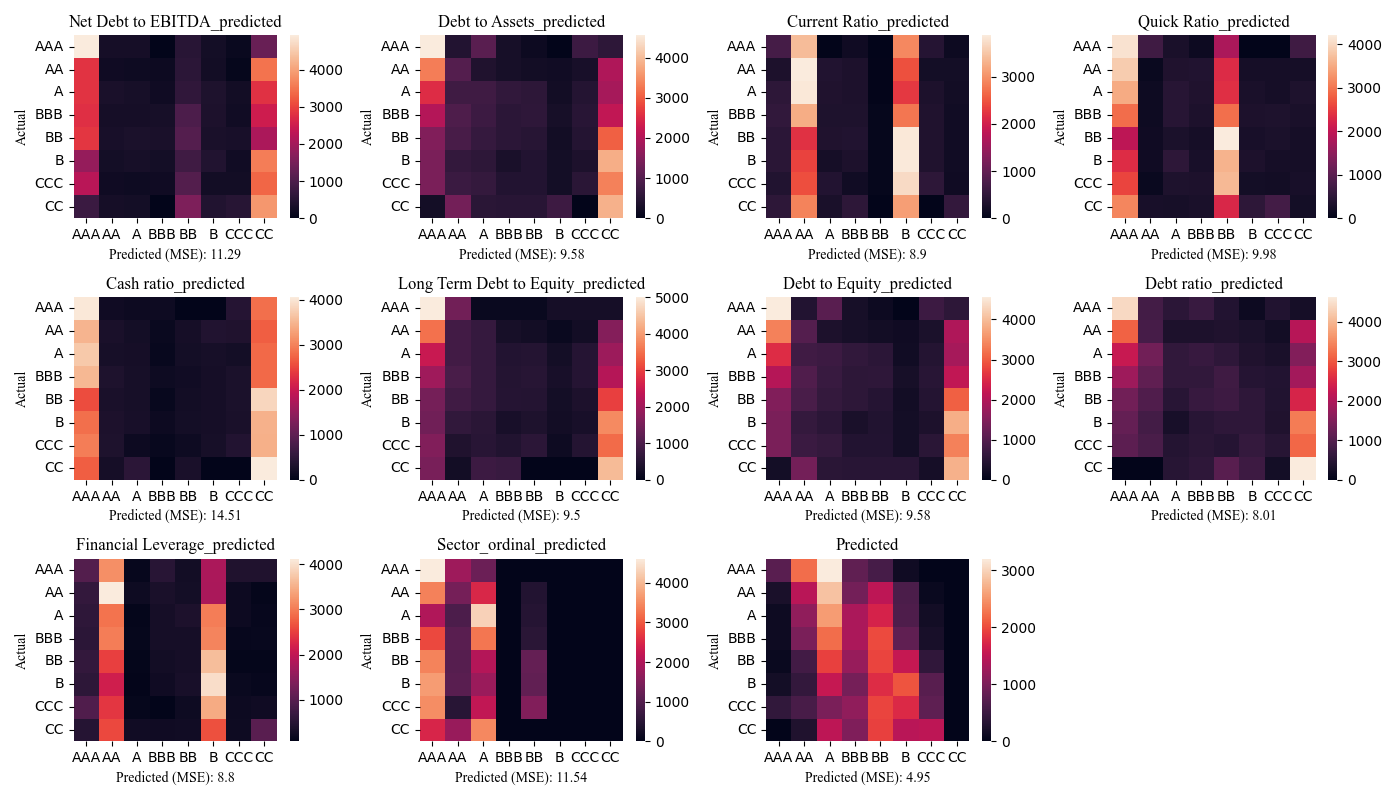
\includegraphics[width=1\textwidth]{confusion_matrix_por_metrica.png}
\caption{Matriz de confusión para cada una de las métricas y la media general.}
\label{fig:confusion_matrix_por_metrica}
\end{figure}

\subsection{Modelos de regresión}

Para estimar nuestro Rating partiendo de las métricas financieras hemos utilizado tres tipos de modelos:
\begin{enumerate}
    \item \textbf{Regressión Lineal}: La regresión lineal es uno de los métodos más simples y ampliamente utilizados para modelar la relación entre una variable dependiente y una o más variables independientes. El objetivo es encontrar en el hiperplano que mejor se ajuste a los datos, minimizando la suma de las diferencias cuadradas entre los valores observados y los valores predichos por el modelo. La forma general de la regresión lineal para una variable dependiente \(y\) y \(n\) variables independientes (\(x_1, x_2, ..., x_n\)) es:
    
\[ y = \beta_0 + \beta_1x_1 + \beta_2x_2 + ... + \beta_nx_n + \epsilon \]

Donde \(\beta_0\) es el término de intercepción, \(\beta_1, ..., \beta_n\) son los coeficientes que representan el peso de cada variable independiente en la predicción de \(y\), y \(\epsilon\) es el término de error. Como observamos en la Figura \ref{fig:confusion_matrix_linear_regression} con este modelo obtenemos los peores resultados.

\item \textbf{Regresión Polinómica de grado 3}: La regresión polinómica es una forma de regresión lineal en la que la relación entre la variable independiente \(x\) y la variable dependiente \(y\) se modela como un polinomio de grado \(n\). En este caso las características de entrada son elevadas a potencias hasta el grado 2 (incluyendo combinaciones de características)\footnote{Ya que las métricas suelen emporar de manera exponencial con el Ratings, ya que el salto de calidad crediticia entre AAA y AA+ en mucho menos que entre BB- y B+.}, lo cual permite modelar relaciones no lineales entre las variables. Por ejemplo, para una única variable independiente \(x\), el modelo polinómico de tercer grado sería:
\[ y = \beta_0 + \beta_1x + \beta_2x^2 + \epsilon \]
En este modelos el MSE observado en la Figura \ref{fig:confusion_matrix_polyreg_model} se reducen considerablemente.
\item \textbf{Modelos Logístico}: La regresión logística ordinal es útil cuando la variable dependiente es ordinal, es decir, cuando las categorías tienen un orden natural pero las distancias entre categorías no son necesariamente iguales. El modelo LogisticAT asume que hay un único conjunto de coeficientes (similar a la regresión logística multinomial) pero difiere en que los umbrales para decidir entre categorías consecutivas no son equidistantes. El enfoque busca minimizar una función de pérdida que penaliza la clasificación incorrecta de las observaciones, con el objetivo de establecer umbrales que mejor separen las categorías en orden.
\end{enumerate}

\begin{figure}[H]
    \centering
    \begin{minipage}[b]{0.32\textwidth}
        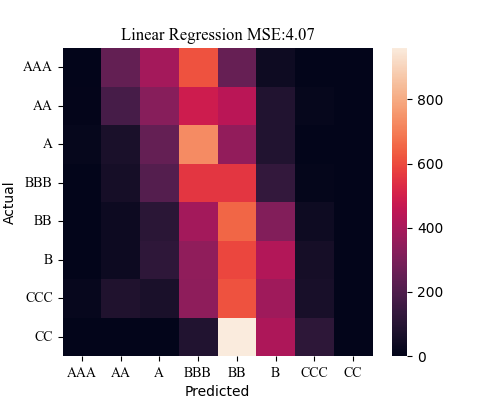
\includegraphics[width=\textwidth]{confusion_matrix_linear_regression.png}
        \caption{Regresión Lineal}
        \label{fig:confusion_matrix_linear_regression}
    \end{minipage}
    \hfill % Espacio opcional entre figuras
    \begin{minipage}[b]{0.32\textwidth}
        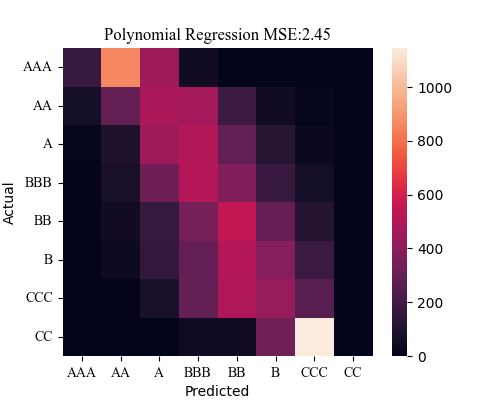
\includegraphics[width=\textwidth]{confusion_matrix_polyreg_model.png}
        \caption{Regresión Polinómica}
        \label{fig:confusion_matrix_polyreg_model}
    \end{minipage}
    \hfill % Espacio opcional entre figuras
    \begin{minipage}[b]{0.32\textwidth}
        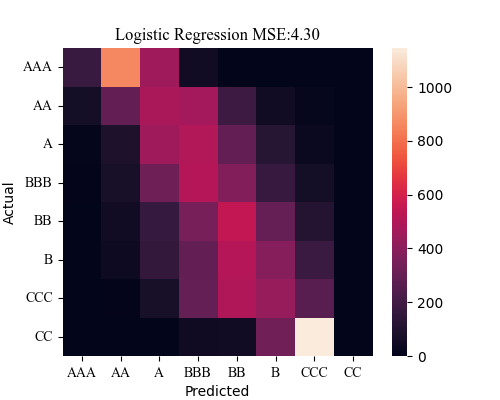
\includegraphics[width=\textwidth]{confusion_matrix_logistic_model.png}
        \caption{Regresión Logística}
        \label{fig:confusion_matrix_logistic_model}
    \end{minipage}
\end{figure}

\subsection{Modelos de ML}

Por último hemos creado un modelo Randam Forest (Bosque Aleatorio) de ML. Este modelo de Machine Learning es un método de ensamble que opera construyendo múltiples árboles de decisión durante el entrenamiento y produciendo la clase que es la predicción media de los árboles individuales. Este método se basa en combinar las predicciones de varios arboles de decisión de aprendizaje automático para hacer predicciones más precisas que cualquiera de los modelos individuales. A continuación explicamos algunos de los puntos más importantes del Borque Aleatorio.

\begin{enumerate}
    \item \textbf{Árboles de decisión:} Son la unidad básica de un Random Forest. Un árbol de decisión es un modelo que hace predicciones siguiendo una serie de reglas de decisión binarias (sí/no) basadas en las características de los datos. Aunque poderosos, individualmente, los árboles de decisión pueden ser propensos al sobreajuste.
    \item \textbf{Ensamblaje (Bootstrap Aggregating o Bagging):} Para crear un Random Forest, primero se genera una serie de árboles de decisión. Cada árbol se entrena con una muestra aleatoria de los datos de entrenamiento, seleccionada con reemplazo, conocida como bootstrap sample. Esto ayuda a asegurar que cada árbol sea diferente y reduzca el riesgo de sobreajuste.
    \item \textbf{Aleatorización:} Además de la aleatorización introducida por el bootstrap sampling, Random Forest introduce más variabilidad en los árboles de decisión al limitar el conjunto de características que se pueden considerar para dividir en cada nodo de los árboles. Esto significa que, en lugar de buscar la mejor característica al dividir un nodo, el algoritmo busca la mejor característica entre un subconjunto aleatorio de características. Esto hace que los árboles sean más diversos y mejora el rendimiento del modelo general.
    \item \textbf{Agregación:} Después de entrenar, las predicciones de todos los árboles individuales se combinan para formar la predicción final. Para problemas de clasificación, esto suele significar tomar la moda (la clase más frecuente) de las predicciones de todos los árboles. Para regresión, se toma el promedio de las predicciones.
\end{enumerate}

Dividiendo nuestros datos en dos conjuntos de Train y Test hemos entrenado el modelo de Random Forest con únicamente 3 Árboles de decisión, obtenindo un acierto en el 93\% de los casos. Sin embargo, en la sección \ref{sec:resultados} analizaremos este modelos con más detalle.

\begin{table}[H]
    \centering
    \begin{tabular}{|l|c|c|c|c|}
    \hline
        Tipo de regresión & Aciertos exactos & Acierto ($\pm 1$ ) \\  \hline
        Regresión Lineal & 17,25\% & 49,61\% \\ \hline
        Regresión Logística & 18,33\% & 51,67\%  \\ \hline
        Regresión Polinomial & 19,13\% & 54,42\%\\ \hline
        Random Forest \footnote{Este modelo no ha usado el rating agrupado, si no que hemos empleado como variables dependiente los Ratings definidos por S\&P.} & 89,66\% & 92,21\%\\ \hline
    \end{tabular}
    \caption{Precisión de las estimaciones}
    \label{tab:aciertos}
\end{table}

\section{Resultados}\label{sec:resultados}

Como hemos mencionado anteriormente, al haber realizado un \textit{oversample} de nuestra muestra, cuando hacemos las estimaciones con datos diferentes a los que el modelo usa para entrenar, no podemos asegurar que sean datos diferentes, ya que para algunos Ratings, la muestra original era varios ordenes de magnitud menor que para la categoría más frecuentes, como observamos en la Figura \ref{fig:dist_rat_sec}.

Por comprobar la eficacia del modelo, hemos sacado todas las métricas para los principales índices del mundo para el año 2024, para asegurarnos que tenemos datos que nunca han pasado por el modelo. De esta manera obtenemos un buen indicador de la precisión de cada uno de los modelos. Aplicando los mismos filtros y la misma enumeración para las variables categóricas que en nuestro datos originales, llegamos a una muestras de 753 empresas. En la Tabla \ref{tab:aciertos} observamos que el mejor modelo para las 3 medidas de error que hemos calculado es el modelo de Random Forest. Por tanto, hemos realizado las estaimciones con el modelo de Random Forest y representado la matriz de confusión para el modelo de Random Forest en la Figura \ref{fig:confusion_matrix_rf_new_data}. La cual muetra unos resultados bastante buenos, con un acierto en el 54\% de los casos y con una acierto aproximado con +/- 2 Ratings en el 74\%.

\begin{figure}[ht]
\centering
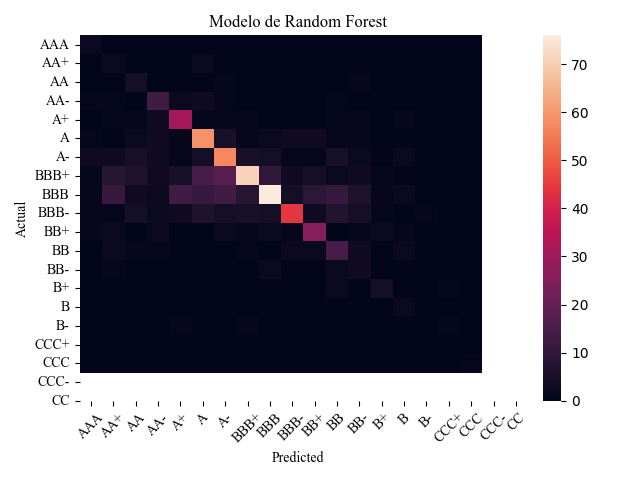
\includegraphics[width=0.6\textwidth]{confusion_matrix_rf_new_data.png}
\caption{Matriz de confusión para los nuevos datos y el modelo de Random Forest.}
\label{fig:confusion_matrix_rf_new_data}
\end{figure}


\section{Conclusiones}\label{sec:conclusiones}

Después de analizar los datos y realizar diferentes tipos de modelos, podemos concluir que mediante los modelos de regresión y clasificación ``clásica'' obtenemos niveles de precisión en nuestras estimaciones aceptables, pero que esta precisión aumenta considerablemente con el modelo de ML de Random Forest. Este trabajo, podría dar pie a una sería de trabajos que analizaran con más profundidad algunos aspectos que no hemos analizado en este trabajo pero podrían mejorar las estimaciones del Rating para algunas compañías. Entre estos trabajos se encuentran:
\begin{enumerate}
    \item Realizar este mismo análisis añadiendo otras métricas financieras, tales como:
    \begin{itemize}
        \item Coste de la financiación.
        \item Capitalización de mercado.
    \end{itemize}
    \item Intentar normalizar los datos para ver si los modelos de regresión reducen su error.
    \item Estudiar si hay diferencia entre las métricas para cada año, ya que nosotros hemos usado datos de diferentes años y esta podría ser una variable a tener en cuenta.
    \item Ver si hay diferencias estadísticas entre las métricas por países y si esta podría ser otra variable independiente.
    \item Analizar si nuestro error de predicción varía por países o por sector.
    \item Aplicar otras técnicas de ML.
    \item Estudiar algoritmos de clasificación no supervisados, para poder clasifique todas las empresas sin Rating.
    \item Buscar versiones de los modelos de ML más sencilla para poder exportar estos modelos a aplicaciones como \textit{Excel}, de manera que sea más accesible para otros usuarios.    
\end{enumerate}


\printbibliography % Imprime la bibliografía


\end{document}